\chapter{Visual Diffing a CPS in a Virtual World (15 Pages)}

\section{Problem}
\label{sec:Problem}
Testing a CPS in either simulation and the real-world typically involves recording data to logs, before then reading and processing (using tools or custom scripts) the logs off-line, in order to analyse, discover and diagnose issues. Simulation tools provide the possibilities to record more data due to the increased access and lack of constrained hardware, however, are still limited in how they can present it to users, still heavily relying of textual logs.

Processing log data manually is extremely time-consuming and only provides limited context given the amount of information a developer can read and process at one time. Utilising scripts or external analytical tools can provide more intuition about the data in significantly less time, however, results are provided off-line and outwith the context of the experiment.

Testing in the virtual world provides developers with access to significantly larger volumes of data about a simulation than is possible to record from the real world, including information about entities in the world and the physical environment; combined with a fully customisable and controllable 3D world, this opens up the possibilities to more advanced and visually integrated analytical tools. 

However, this benefit comes at a cost. Firstly, with such large volumes of data, at the rate of gigabytes per hour, how can developers process, analyse and make use of all the data in real-time, without resorting to reading and parsing logs? Secondly, using this data, how can developers visually compare and contrast two or more simulations, to identify differences when performing A-B testing?

\begin{itemize}
  \item Data Volume, how to compress and index in real-time or faster
  \item Visual Bandwidth, how do we show data - how much can we show
  \item How can we compare two streams in real-time
\end{itemize}

\section{Visual Diffing}
\label{sec:visualDiffing}
Understanding differences between two or more entities is a common but vital task across variety of domains, including text, image, voice and video analysis. System administrators or developers who need to know the differences between two text files employ the `diff' UNIX tool\footnotemark, which highlights lines that don't match between files; Doctors and medical staff compare medical scans, often overlaying one onto the other with a backlight, to spot key differences; In sports, video replays are combined to show two or more racers simultaneously (Dartfish), or utilise high-speed multi-camera arrays to generate 3D models to discover if tennis shots are out of bounds (Hawk-eye).
\footnotetext{From which the term visual diffing is coined.} 

Inspired by its use in other domains, visual differencing, ``visual diffing'' for short, enables viewers to observe the both visible and non-visible differences between two or more instances of an event incorporated directly into the visual medium itself. This contrasts to overlaying abstract data metrics, such as speed or time, over a video, image or simulation, requiring viewers to consciously analyse. Instead, visual diffing utilises visual techniques and clues integrated into the scene which enable viewers to intuitively visually observe differences and areas of interest without needing to remember and compare abstract metrics.

Whilst not formally described as visual diffing in other domains, techniques which can be described as such can be found in sports coverage and a variety of other media, shown in figure \ref{fig:visual_diff_sports}.

\begin{figure*}[th!]
\subfloat[The Hawk-Eye system showing where all service shots for a player land within the court.]{
	\centering
	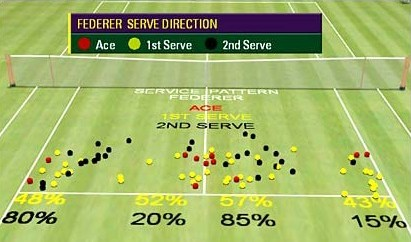
\includegraphics[width=0.49\textwidth]{img/hawk_eye_visual_diff.jpg}
	\label{fig:hawk_eye}
}
\hfill
\subfloat[The Hawk-Eye system showing the path a shot took, to help determine if it is at fault.]{
	\centering
	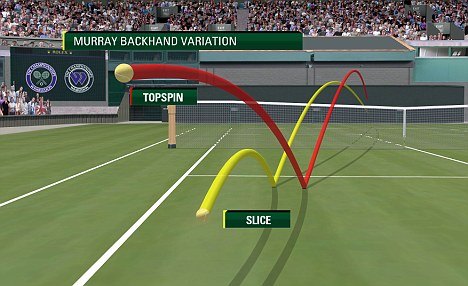
\includegraphics[width=0.49\textwidth]{img/hawk_eye_paths.jpg}
	\label{fig:hawk_eye_path}
}

\subfloat[The Hawk-Eye system showing a heat map of player positions so far.]{
	\centering
	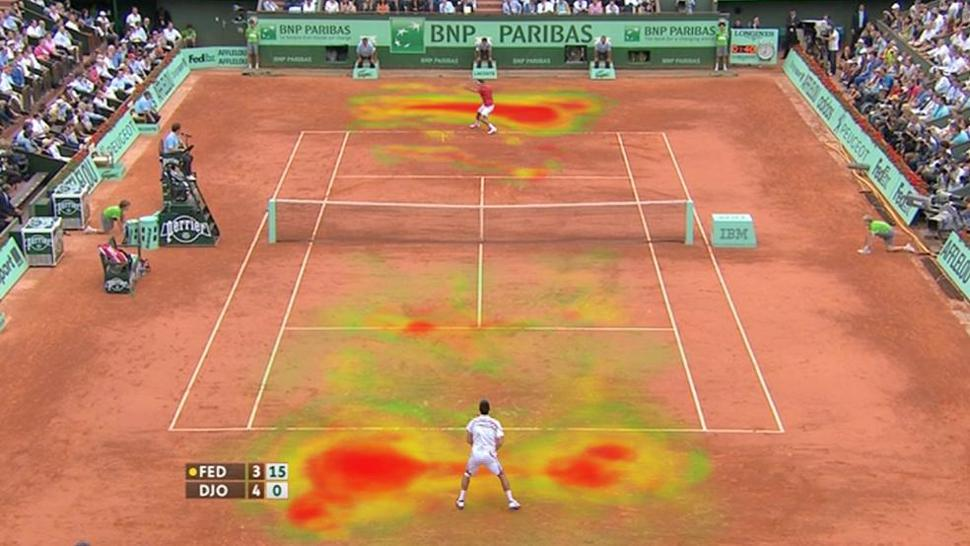
\includegraphics[width=0.49\textwidth]{img/hawkeye_heatmap.jpg}
	\label{fig:hawkeye_heatmap}
}
\hfill
\subfloat[Dartfish simulcam ski racing, showing three individual racer's time trials combined into one replay.]{
	\centering
	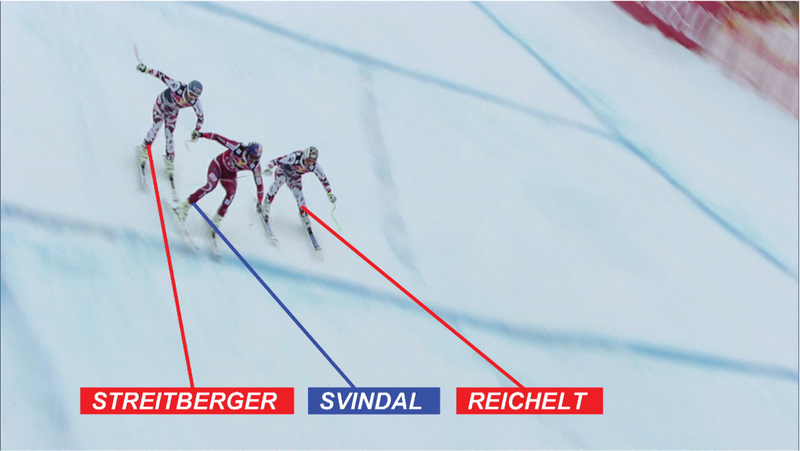
\includegraphics[width=0.49\textwidth]{img/dartfish_simulcam_visual_diff.jpg}
	\label{fig:dartfish}
}

\caption{Examples of Visual Diffing within sports replays.}
\label{fig:visual_diff_sports}
\end{figure*}

\subsection{Techniques} % (fold)
\label{sub:techniques}
The simplest of visual diffing techniques show spatial differences between entities in a scene, enabling observers to interpret the distance and difference in speed. Depending on the medium, image or video, different techniques are more affective for presenting information. Other techniques can help better translate non-visible data metrics, such as acceleration, speed, type, etc, to physical attributes, such as size and colour. 

A non-exhaustive list of visual diffing techniques commonly used include:

\textbf{Ghosts}\footnotemark, a common technique used in sports, in which two or more people or objects occupy the same on-screen environment, enabling visual comparisons of differences in position, speed and movement of participants. For example, shown in figure \ref{fig:dartfish}; two individual slalom skiers racing in time-trials, are visually overlaid as ghosts onto the same race track. This provides viewers with a visually exciting but also intuitive experience as the race progresses, without the need to resort to just time metrics. 

\footnotetext{The name ghosts comes from the ability of entities to pass through objects and each-other unaffected, not necessarily their ghastly colour, which is added to aid in disambiguation in DejaVu.}

\textbf{Paths}, provide a visual history of where a person or object has been within an environment, typically represented as a line. Where ghost provides visual intuition at a discrete time-slice, paths provide it over a continuous time period. Within a slalom race, this enables viewers to observe what line a racer takes when skiing down a race course. These paths can be overlaid with others to compare racers directly, or even combined with ghosting to add more visually intuitive elements for the user to understand how a race progresses.

\textbf{Colour + Size}, enables non-visual data to be presented via a visual medium. Colour and size can be used to display both discrete and continuous data, providing more information or highlighting hidden points of interest typically missed e.g., a set of colours can denote states, such as red, yellow and green, or a gradation of colour and size can be used to signify the strength or intensity of a data. Figure \ref{fig:hawk_eye} utilise colour to provide meta-data about different tennis serves, whether they were first, second or ace serves. 

\textbf{Heatmaps}, show the frequency of an entity or an action being carried out at a specific location within a space, through colour intensities displayed over a map. This provides at a glance where hot- and cold-spots of activity are within an environment, enabling viewers to instantly locate areas of interest. Figure \ref{fig:hawkeye_heatmap} shows a heatmap overlayed on a tennis court, showing where the tennis players have returned shots since the start of the match, with higher frequency areas show increasingly intense colours, from green to yellow to red. Heatmaps are very effective for showing accumulative data  

% subsubsection techniques (end)

\section{Implementing Visual Diffing} % (fold)
\label{sec:implementing_visual_diffing}
Implementing visual diffing techniques utilises the recording framework described in section \ref{sec:recording}.

\subsection{Ghosts} % (fold)
\label{sub:ghosts}
The ghost visual diffing technique is the simplest technique visually, making it possible to view two simulation replays simultaneously in the same environment, with one simulation's entities rendered as solids whilst the second's are ghosts, shown in figure \ref{fig:cps_diff}.

\begin{figure*}[h]
    \centering
	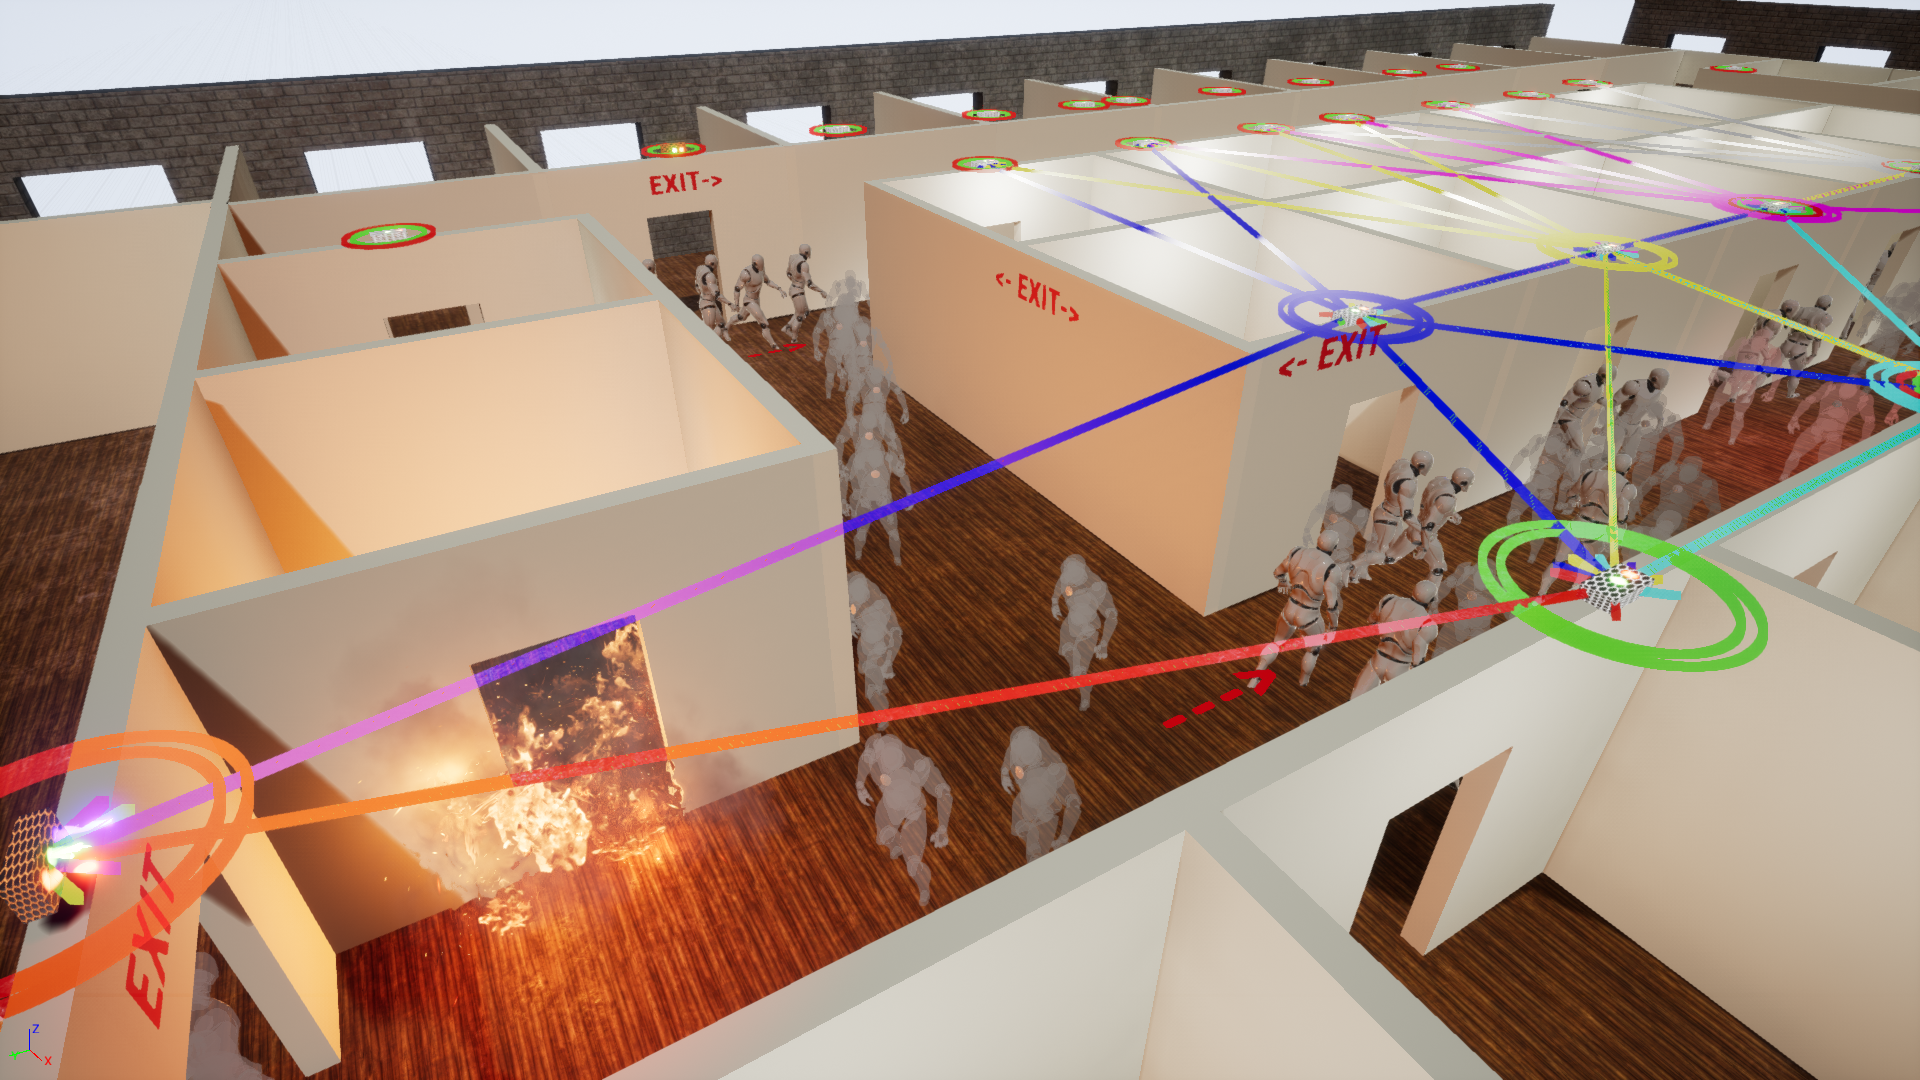
\includegraphics[width=0.8\textwidth]{img/fireEvacCPS2.png}
	\caption{CPS-enhanced evacuation diffed with non-enhanced ghosts. Evacuees are being directed to exits via safe routes.}
	\label{fig:cps_diff}
\end{figure*}
% subsection ghosts (end)
The simulator supports visual diffing a live simulation against a recorded replay, or one recorded replay against another. When visual diffing is enabled, the simulator creates ``ghost'' entities corresponding to the entities in the recorded repla,y which play out the recorded data from the replay. ``Ghost'' entities are not created for static objects in the environment, such as walls or floors - as these objects can't move.

In order for the ``ghost'' visual diffing technique to work, ``ghost'' entities must have a corresponding ``live'' entity (from the simulation or corresponding replay), so that the diff can be observed. ``Ghost'' and ``live'' entities are linked via id tokens. ``Ghost'' entities don't physically interact with the live simulation, simply replaying what was originally recorded. As the live simulation is run the the simulation time ticks at 60FPS; at each simulation tick the replay time updated and any snapshots that need to be applied are applied to the ``ghost'' entities.



% section implementing_visual_diffing (end)
\subsection{Paths} % (fold)
\label{sub:paths}
The path visual diffing technique displays the movement history of a entity as it traverses through the environment, leaving behind a trail consisting of lines and spheres, shown in figure \ref{fig:path_navigation_diff}.

Paths are generated in real-time from a recording, starting from time \textit{t0}, a time sphere is created for each movable entity. New spheres are created at 1-second intervals, to reduce the granularity and provide visual time-step clues, joined by a line. Using this combination of spheres and lines provides a visual path of where an entity has been and the rate at which they were travelling. This makes it trivial to observe movement patterns and changes between different simulation runs.

For fast moving entities, it is possible decrease the interval time to increase the path granularity, displaying smoother paths through the environment.

The time spheres also provide a secondary time traversal function, time warping, described in section \ref{sub:time_spheres}.

\begin{figure}[h]
	\centering
	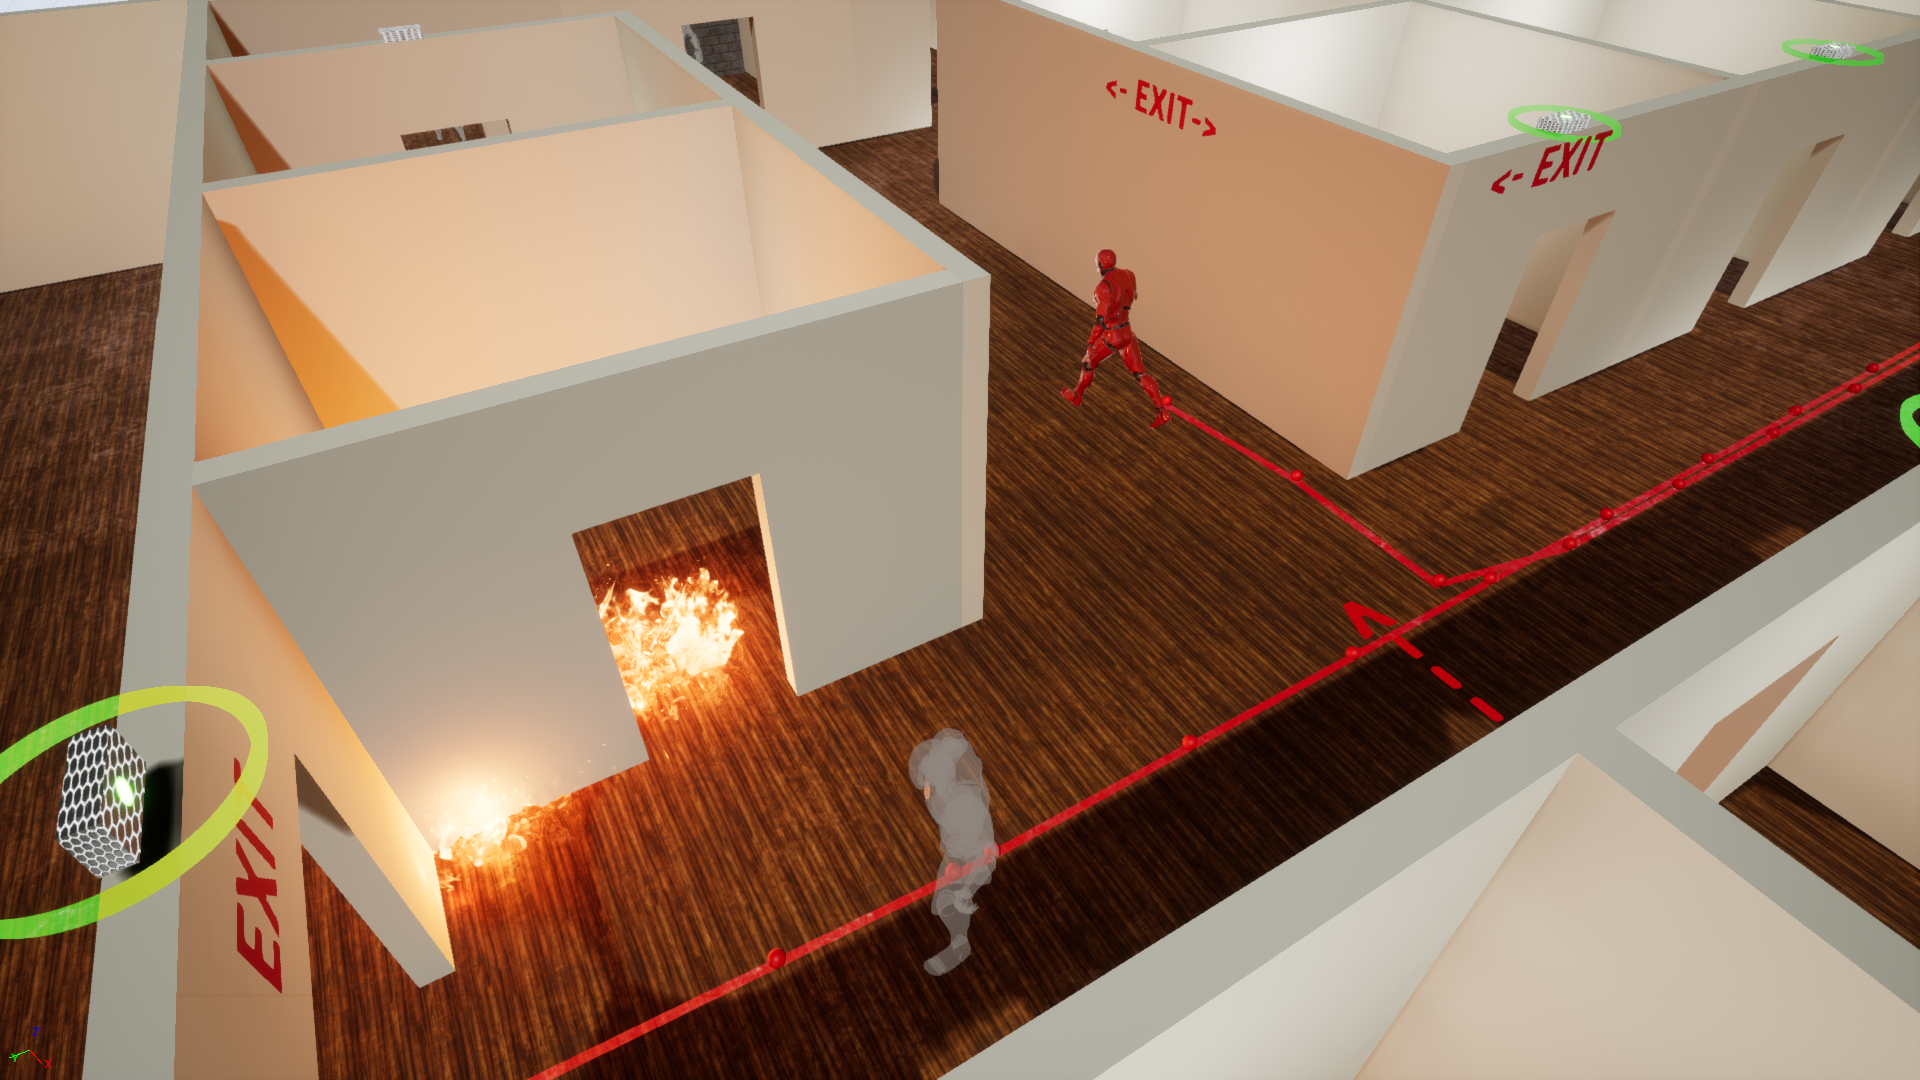
\includegraphics[width=0.8\textwidth]{img/fireevacghost.png}
	\caption{A person evacuating chooses two different paths in different runs based on CPS assistance, the ghost shows the same person taking a different route in a previous run.}
	\label{fig:path_navigation_diff}
\end{figure}
% subsection paths (end)

\subsection{Time Warping} % (fold)
\label{sub:time_spheres}
Time Spheres provide a secondary time traversal tool for visual diffing, time-warping. Within the virtual world times spheres are interactive, allowing observers to click on them to instantly time-warp between different time points. 

As time spheres are generated they contain a reference to the time point at which they were created. Using this time point reference, the simulator can find and load the appropriate snapshot, resetting the environment to that snapshot's state. When this happens, the paths and time spheres remain, allowing for observers to time warp back and forth between time points.

% subsection time_spheres (end)
\subsection{Colour and Size} % (fold)
\label{sub:colour_and_size}
Ghosts and path visual diffing techniques support visualising spatial differences between entities, making it simple to spot differences over time or between simulations. However, visual diffing of internal state or non-visual data requires more creative visual techniques, such as colour and size.


\begin{figure}[h]
	\centering
	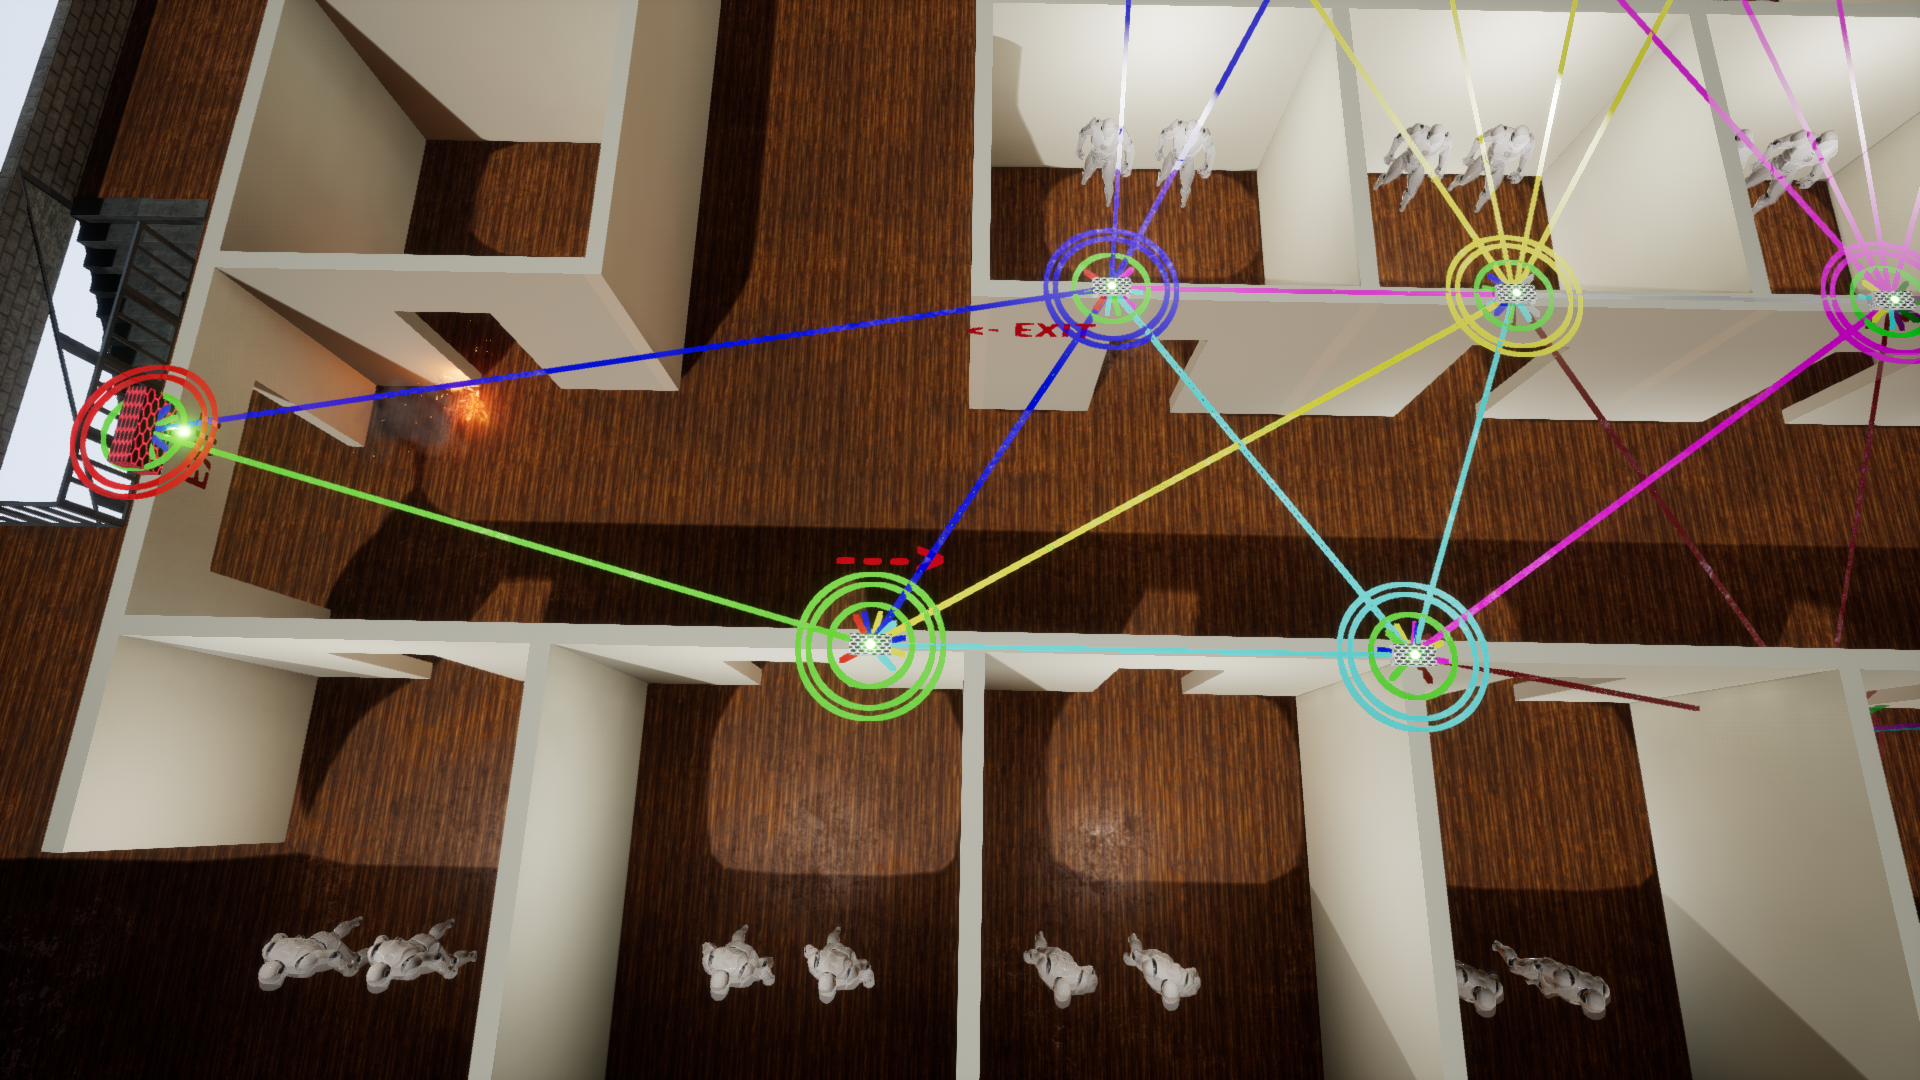
\includegraphics[width=0.8\textwidth]{img/biggerSensorAlert.png}
	\caption{One of the sensors is red in colour and enlarged, representing a change in state when diffed to another run.}
	\label{fig:diff_colour size}
\end{figure}
% subsection colour_and_size (end)
\section{Recording and Time Control}
\label{sec:recording}
Running and recording CPS tests in real-world deployments is a difficult and time-consuming task, requiring not only recording and retrieving logs from a network of devices, but also video recording environments when physical phenomena are involved, such as people interacting with the system. Recording in the real-world is a ``one-shot'' chance, where anything missed, due to not being recorded in a log or within the video frame, can't be retrieved, requiring either guesstimating or a test re-run. Recording large volumes of data on-device may not be possible due to the constrained hardware, similarly, the network bandwidth may not support such data either, not without having adverse affects on the rest of the CPS. 

Running simulations in a 3D virtual world opens up the opportunity for recording reconstruct-able replays, utilising data recorded from both the CPS simulation and from virtual world. Unlike other real-world or simulation recording approaches, these reconstructed replays allow viewers to see the cyber-physical cause and effect after-the-fact. Similarly, by recording at the simulation level, application code doesn't need to be edited to support it, ensuring application logic and control-flow consistency is guaranteed between testing and deployment.

Providing this level of replayability enables more comprehensive post-simulation review and analysis. For real-world deployments, simple video recordings which may be carried out and are limited to the recorded view(s) and are read-only once recorded. Instead, by recording reconstructions, viewers are able to manipulate time and space within replays, pausing, fast-forwarding and replaying events from any angle within the scene. Reconstructions also allow for analytics to be seamless added to or removed from the replay in real-time, such as ghosts, providing a dynamic and flexible tool-kit e.g., changing viewing angles/position and altering what visual diffs are applied.

Recording long-term simulations provides different challenges, not only requiring efficient storage of the reconstruction, but also how to efficiently access, index and review the points-of-interest. Solving these issues opens up the opportunity to run longitudinal CPS studies for testing robustness and reliability, even against running systems e.g., a real running system could run parallel to a upgraded simulated version, feeding inputs and testing whether the new version maintains the same functionality.

\begin{itemize}
  \item Gigabytes of data per hour, how to store, compress, index...
  \item Synchronising recordings, replay, rewind, fast-forward efficiently.
\end{itemize}

\subsection{Recording Data} % (fold)
\label{sub:recording_data}
Simulation within the co-simulation platform targets 60FPS to provide a smooth and responsive simulation. Thus, recording enough data to support creating reconstructions matching the original run requires logging the attributes of every entity within the world and CPS simulator at 60x per second, including location, rotation, speed and other entity-specific internal state. This can generate GBs of data per hour without optimisation, limiting simulation recordings to several hours on an average workstation.

The following sections describe several optimisations and techniques used to improve the space-saving yield whilst maintaining the smooth performance.
% subsection recording_data (end)
\subsubsection{Raw} % (fold)
\label{sub:raw}
In order to record full reconstructions, the simulator needs to record both visible and non-visible behaviour i.e., both physical and internal state. Such data includes, position, rotation, trajectory, sensor data, transmission state, etc. By ensuring as much information as possible is stored, future reviews are able to view and process not just what developers thought might have been necessary when they ran the test. However, this extra information comes at a cost, as shown in figure \ref{tab:recording_costs}.

At each time slice, a snapshot of an entity's state is stored as part of its history, in chronological order starting from time \textit{t0}. Thus, in order to rewind to a previous state, the simulator simply sets the entity's state equal to the snapshot. For moving to a specific time point, the simulator uses the time stamp as an index to locate the correct snapshot, then simply sets the state to that.
\sidenote{Revisit how it moves to a specific time point}

\begin{table}
	\centering
	\caption{Recording costs of objects within the simulator}
	\begin{tabular}{|c|c|c|c|}
	\hline
	Data & Size & 1min Total & 1hr Total\\\hline
	Location & 16Bytes & 56KBytes & 3.2MBytes\\\hline
	Rotation & 16Bytes & 56KBytes & 3.2MBytes\\\hline
	Scale & 16Bytes & 56KBytes & 3.2MBytes\\\hline
	Velocity & 16Bytes & 56KBytes & 3.2MBytes\\\hline
	Angular Velocity & 16Bytes & 56KBytes & 3.2MBytes\\\hline
	Time Stamp & 4Bytes & 1.4KBytes & 84KBytes\\\hline
	Sensor State & 39Bytes & 137KBytes & 8MBytes\\\hline

	\end{tabular}
	\label{tab:recording_costs}
\end{table}
% subsubsection raw (end)

\subsubsection{Optimisations} % (fold)
\label{sub:compressed}
To reduce the amount of data recorded, instead of storing a snapshot of an entity at every tick (60FPS), we can instead store one only when some or all of its state has changed, thus saving considerable amount of space for entities which become inactive, physically or virtually; however, for simulations where all entities are active, the savings may be limited. 

When using this technique, searching for specific time points becomes more difficult as there may not be a corresponding snapshot for an entity, instead the last recorded snapshot before the requested time point should be used.

To further improve upon this, each snapshot only contains what has changed between time slices, starting from time \textit{t0}. When rewinding or fast-fowarding through a continuous time period, these delta snapshots can be applied like before, except updating only the changed state. 

However, providing random access to the history becomes more difficult, due to the snapshot containing only what has changed, if any snapshot exists at all for that time point. To jump to time \textit{tn}, the simulator must start from \textit{t0} and apply each delta snapshot up to \textit{tn}, resulting in an O(n) time. Alternatively, at a set interval -- checkpoint, a full snapshot could be stored, enabling faster state restoring, requiring finding the nearest checkpoint to time \textit{tn}, before then applying each update until reaching \textit{tn}. This reduces the time to O(n/m), where m is the number of checkpoints, thus, a higher number of checkpoints reduces the search time, but will increase the storage consumption.

\TODO{Run experiment to see difference between optimisation and compression}
\begin{table}[h]
\centering
\caption{Size comparison between raw and compressed snapshots saved to disk, varying in length.}
\begin{tabular}{|l|l|l|l|l|l|}
\hline
           & 1min  & 1hr    & 24hr  & 7days\\ \hline
raw        & 40MB  & 1.5GB  & 36GB  & 252GB\\ \hline
optimised  &\textbf{TODO}&\textbf{TODO}&\textbf{TODO}&\textbf{TODO}\\ \hline     
compressed & 1.6MB & 45.1MB & 1.1GB & 8GB\\ \hline
\end{tabular}
\label{tab:offline-storage}
\end{table}
% 7 252GB 8GB
% 10mins 30mins   47mins
% r 272.4MB 834MB 1.25GB
% c 8MB 24.5MB    36.5MB
% subsubsection compression (end)

\subsection{Enabling long-term recordings} % (fold)
\label{sub:enabling_long_term_recordings}
With the current recording solution, even with the delta optimisation, it's possible to run out of memory within a few hours, if a given scene has many entities which are all very active, moving and changing state regularly. Therefore, to record, replay and analyse long-term CPS simulations consisting of days or weeks of content further improvements are needed to provide efficient loading, viewing and storing of these recordings. 

The rest of this section discusses several techniques employed to improve performance and usability when using long-term recordings.

\subsubsection{Snapshot Chunking, Compression and Time-Shifting} % (fold)
\label{sub:chunked_compression}
Currently, when viewing a replay sequentially, the replay file can be streamed into memory, providing O(1) access to replay content. However, the current format doesn't support random access, requiring the whole replay to be loaded into memory up to the time point of interest, O(n) time, where n is the time point. This is not an optimal solution given replays can be in the order of hours to days.

When replaying a long replay the system needs to sequentially load in the recording until the desired time-point is reached. This makes viewing small segments of hour/day/week long simulations inefficient. 

To solve this, snapshot chunking is used. The continuous stream of snapshots both full and deltas, are divided into chunks or segments of a fixed size. Segments which are not currently being viewed are compressed and written to storage (disk or ssd). When running a replay the initial segment is loaded and the rest of the segments are set to lazy load in on-demand. This technique significantly reduces the memory requirements for recording and viewing long term recordings.

Compression is used to significantly reduce the size of segments whilst on-disk. As segments are saved to or loaded from disk they are compressed or uncompressed, respectively. 

Because of the optimisations used for storing snapshots, equal length time slices can contain significantly different numbers of snapshots, which would result in vastly different snapshot sizes e.g,. fixed 30sec snapshots: snapshot 1 contains 100 snapshots, whereas due to inactivity snapshot 2 and 3 contain only 20 snapshots each. This causes unpredictable loading performance and memory usage when accessing and de-compressing segments, with smaller segments loading quickly versus larger ones taking significantly longer and consuming considerably more space. Alternatively, storing fixed size segments ensures predictable memory usage and loading speed.

Pre-emptive segment loading is used to improve sequential and short-distance time-shifting performance i.e., segments before and after the current segment are loaded. This allows the user to jump forwards or backwards crossing into adjacent segments without causing significant slow downs caused by waiting for segments to be loaded in from disk. The number of pre-emptive segments loaded can be adjusted based on the available memory and performance requirements.

Utilising these techniques makes long-term recordings feasible, significantly reducing the space and time required to store, load and view recordings, from over a gigabyte for 1 hour to under 50 megabytes.  

\begin{figure}[ht]
\centering
  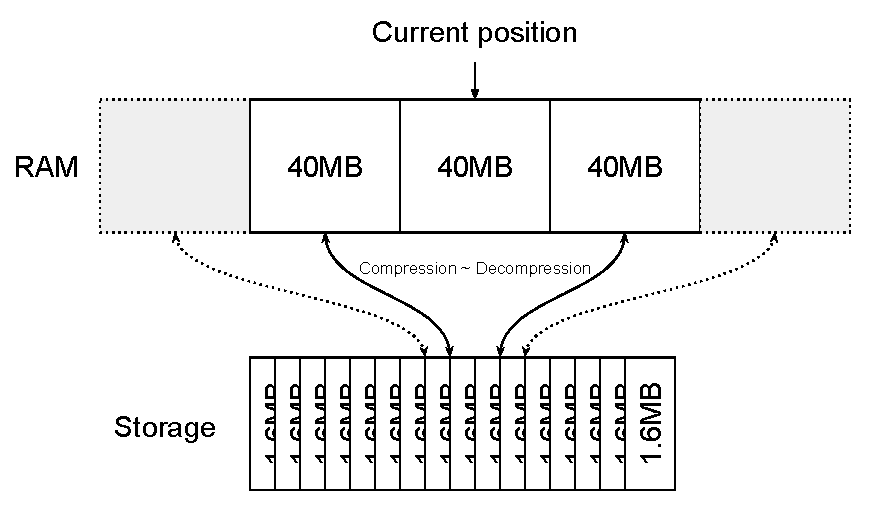
\includegraphics[width=0.75\textwidth]{img/DejaVuCompression.pdf}
  \caption{Segmented compression scheme employed by DejaVu to reduce in-memory usage.}
  \label{fig:compression}
\end{figure}
% subsubsection chunked_compression (end)


\subsection{Finding Points-of-Interest} % (fold)
\label{sub:indexing_points_of_interest}
Recording, storing and viewing long replays are made possible by the chunked compression recording scheme described above, however, generating this much replay content requires reviewing it too; when reviewing there are often periods of interest when certain activity or no activity may be occurring, but in order to find those interesting points users must watch the footage until they find that point in time, a time-consuming task which defeats the benefit of simulation being faster than real-time. Therefore, some form of automatic indexing of points-of-interest is necessary, enabling developers to instantaneously time-shift there without the need to search.

\subsection{Built-in PoI} % (fold)
\label{sub:built_in_poi}

% subsection built_in_poi (end)
To resolve this issue, we developed a set of built-in listener functions which trigger point-of-interest checkpoints in the timeline when the event of interest occurs. Using this checkpoint developers can time-shift directly to it to see and understand what happened. Using these functions developers can instruct the simulator to watch for certain attributes or events to occur e.g., watch for when node 1 receives a message, when a person is moving/stops moving.

These functions are set to run once per tick to access the necessary simulation data and determine if a condition has been met. These functions include checking: when a node transmits, when a node moves, when a nodes LED state changes, when a PIR sensor has been triggered.

Ideally developers should be able to write functions which can access the event stream and then generate custom PoI checkpoints.

% subsection indexing_points_of_interest (end)
\subsubsection{Pub/Sub PoI} % (fold)
\label{sub:pub_sub_poi}
Because the framework is built upon a Pub/Sub message bus, it makes it possible for external tools to subscribe to the simulation event stream, perform stream processing and pattern match for events of interest. Using this developers can write custom event watchers without recompiling the simulator code.

To make this work the simulation components publish world and simulation events to the message bus, to which external components can subscribe. The simulator also subscribes to the PoI stream; when a developer's event listener finds a match it can then publish the timestamp and event name to the PoI stream; when received by the simulation component, it records this PoI checkpoint for later playback.

Utilising this Pub/Sub architectural approach decouples developers from the simulator codebase and language, enabling developers to write custom scripts/tools in larger number of languages and tools.
% subsection pub_sub_poi (end)

% subsection enabling_long_term_recordings (end)
\section{Full Time Control} % (fold)
\label{sec:full_time_control}

% section full_time_control (end)

% section diffing_two_cps_visually (end)
\section{Case Study Analysis}
\label{sec:Case Study Analysis}

\section{Evaluation}
\label{sec:Evaluation}
\begin{itemize}
  \item How does it perform?
  \item Is it possible to compare 2 or more in real-time or even faster?
\end{itemize}

\subsection{Compression} % (fold)
\label{sub:compression}

% subsection compression (end)

\subsection{Real-time Performance} % (fold)
\label{sub:real_time_performance}

% subsection real_time_performance (end)
% subsection  (end)

\section{Conclusion}
\label{sec:Conclusion}
